\documentclass[11pt]{article}

\usepackage[letterpaper, margin=1in]{geometry}

\usepackage[utf8]{inputenc}
\usepackage{graphicx}
\usepackage{cite}
\usepackage{bibentry}
\usepackage{float}

%\pagenumbering{gobble}

\newcommand{\unit}[1]{\ensuremath{\, \mathrm{#1}}}

\title{Laser Control of Electron Spin Resonance: Toward Enhanced Contrast Imaging and Sensing}
\author{Sean Blakley, Joe Becker, Alexsei Zheltikov}

\begin{document}
\begin{center}
\LARGE{Project Description}
\end{center}
\section{Rationale and Objectives}
Recent studies of the energy level structure of the negatively charged nitrogen—vacancy center (NV$^-$) in diamond have 
left much controversy concerning the energy level distribution of the short-lived $^1$A singlet state and the metastable $^1$E singlet state \cite{Goldman2015,Goldman2015a,Toyli2012} (henceforth referred to as the singlet state) within the band-gap 
of the diamond lattice.  The location of these energy states within the band-gap is of fundamental importance in the 
drive to understand the spin-selective shelving process that ultimately underlies most applications of the nitrogen—
vacancy diamond (NVD).  A thorough understanding of the energy level distribution of the NV$^-$ singlet state manifold may 
allow for novel measurement regimes employing spin-selective ionization of the NV$^-$ from the singlet state, affording 
the prospect of enhanced optically detected magnetic resonance (ODMR) contrast for higher sensitivity measurements 
of magnetic fields and temperature distributions.  Another open question is the degree to which the ODMR contrast 
depends on the wavelength of radiation targeted at the infrared (IR) transitions within the NV$^-$ singlet state 
manifold versus its dependence on the temperature of the NVD \cite{Blakley2016}.   There are many open questions regarding the phonon 
sideband structure of the NV$^-$ singlet state that which could be explored using the dependence of ODMR contrast on 
the wavelength of radiation targeted at the IR transitions within the NV$^-$ singlet state manifold.  Knowledge of the 
dependence of ODMR contrast on NVD temperature could facilitate temperature sensitive lock-in detection assisted stimulated emission depletion (STED) imaging using NVD nanoparticles by employing a pulsed microwave source 
targeted at the zero-field ground state sublevel splitting for modulating NVD fluorescence, and using the dependence of the ODMR contrast on temperature to generate super-resolution images with temperature sensitivity.

As a part of the proposed research, we plan to investigate the separation of the NV$^-$ singlet state from the 
conduction band edge by employing a wavelength-dependent photoionization regime involving pulsed microwave and 
wavelength-tunable laser excitation.  The singlet state of an NV$^-$ will be populated through a spin-selective 
intersystem crossing (ISC) with sequential microwave and laser pulses, whereupon a pulse of wavelength-tunable laser 
radiation will be applied to the NV  until it is ionized into a neutrally charged NV center (NV$^0$).  This 
spin-selective photoionization ties the fluorescence excited from the subsequent NV$^0$ to the population in the 
NV$^-$ singlet state as a function of laser wavelength, thereby allowing for determination of the distance of 
the singlet state from the edge of the conduction band by identifying the peak in NV$^0$ fluorescence intensity 
that corresponds to single photon ionization of the NV$^-$ from the singlet state.  In a subsequent section of 
the proposed research, we will utilize the knowledge gained from determining the singlet energy level 
distribution to create a technique for enhanced contrast ODMR imaging of magnetic fields and temperature 
distributions.

We also propose to explore the dependence of the ODMR contrast on both temperature and IR wavelength.  By pumping 
the NV$^-$ into the singlet state with laser radiation and resonant microwave excitation, we can test the dependence of 
the ODMR contrast on temperature by attaching a thermocouple to the NVD and heating the diamond with a heat source 
to generate a plot of ODMR contrast as a function of temperature.  An additional experiment will 
explore the dependence of the ODMR contrast on the wavelength of IR radiation applied to the NV$^-$ while it is in the 
singlet state by fixing the power from an IR source, varying the applied IR wavelength, and generating a plot of 
ODMR contrast as a function of IR wavelength.  By comparing the two plots in these experiments we hope to 
differentiate the effects of IR radiation and temperature on ODMR contrast.  We plan to leverage this information to 
create a novel temperature sensitive STED regime involving fluorescence amplitude modulation with pulsed microwave 
radiation, lock-in detection to suppress the background autofluorescence that plagues many STED techniques, and 
analysis of the thermally induced change in ODMR contrast as a simultaneous measure of the local temperature 
environment.

The proposed research program includes five work packages.  In the first work package, we propose to determine 
the separation of the NV singlet state from the conduction band by using photoionization as a function of applied 
laser wavelengths.  Research within the second work package will be focused on demonstrating enhanced contrast 
ODMR imaging of magnetic fields and temperature distributions using photoionization.  Research within the third 
work package will include incorporation of the enhanced contrast ODMR imaging technique to improve the 
sensitivity of existing fiber-optic NVD probes that enable deep tissue diagnostics of weak magnetic fields and 
temperature distributions of a biological origin.  The fourth work package will develop separate techniques for 
measuring the dependence of the ODMR contrast on temperature and for measuring the dependence of the ODMR 
contrast on the wavelength of IR radiation applied when the NV$^-$ is in the singlet state.  The fifth work package 
will leverage the information gained from the fourth work package to develop a temporally modulated STED regime 
involving modulation of NV$^-$ fluorescence amplitude with a pulsed microwave source and lock-in detection for 
background insensitive super-resolution microscopy with temperature sensitivity.

\section{State of the Art and Motivation}
A NV color center in diamond is a unique solid-state quantum system \cite{Gaebel2006,Dutt2007,Aharonovich2011}, where the electron
spin can be manipulated, polarized, and read out at room temperature using electromagnetic
fields. The electron spin of NV centers in diamond display an extraordinarily long-lived
coherence even at room temperatures, \cite{Gaebel2006,Dutt2007,Aharonovich2011,Childress2006} enabling coherence-control- enhanced quantum data
processing \cite{Dutt2007,Aharonovich2011} and offering much promise as solid-state qubits \cite{Dutt2007,Aharonovich2011,Childress2006,Nizovtsev2005}, single-photon sources \cite{Beveratos2002}
, efficient contrast agents for super-resolution microscopy \cite{Gruber1997}, and photostable, nonbleaching
markers for bioimaging \cite{Gruber1997,McGuinness2011} including high spatial and temporal resolution imaging of neural
activity \cite{Hall2012}. The sensitivity of the electron spin in an NV center to an external magnetic field has
been shown to enable a new approach in magnetometry, allowing weak magnetic fields to be
detected and imaged with an unprecedented spatial resolution and a remarkable sensitivity \cite{LeSage2013,Taylor2008,Maze2008,Balasubramanian2008}
The temperature sensitivity of magnetic-resonance spectra of NV$^-$ \cite{Acosta2010}
has been shown to enable a new modality of optical thermometry, allowing temperature
measurements with a millikelvin accuracy and an unprecedented, nanometer-scale spatial
resolution \cite{Kucsko2013}, thus offering a unique tool for a thermometry of living cells.

The sensitivity of these techniques depends on the value of the ODMR contrast, which
has historically been capped at 30\%. Recently developed techniques involving spin-to- charge
conversion via photoionization and single-shot charge state readout have improved ODMR
contrast dramatically \cite{Shields2015}. However, the charge state readout method in this technique relies on
low excitation power and photon counting, and therefore suffers from shot-noise limited
sensitivity. This limitation can be overcome by a continuous wave ionization regime targeted at
the singlet state ionization wavelength and reading out NV$^0$ fluorescence. Recent work has left
some uncertainty regarding the separation of the singlet state from the conduction band edge \cite{Toyli2012,Goldman2015,Goldman2015a}. 
To redress this uncertainty, a technique for determining the singlet ionization wavelength
must be developed, and singlet ionization must be demonstrated experimentally.  If such a technique could be developed, then it could be used to enhance ODMR contrast by selectively ionizing out of the NV$^-$ singlet state and reading out the fluorescence of the NV$^0$ charge state, whose fluorescence band is well separated from the NV$^-$.  Since the ambient NV$^0$ population is low, any additional NV$^0$ population contributed by the ionization process will produce a high contrast signal in comparison to the background NV$^0$ fluorescence.  This allows for the possibility of an enhanced contrast photoionization assisted ODMR regime.  Due to the higher ODMR contrast, this photoionization ODMR regime can be utilized to enhance the sensitivity of existing NVD magnetometry \cite{Blakley2016a,Blakley2015,Fedotov2014a,Fedotov2014c,Fedotov2014,Fedotov2016} and thermometry \cite{Fedotov2014b,Blakley2016} regimes, including our pre-existing high spatial resolution, high sensitivity fiber-optic NVD magnetometers and thermometers.

While it is a well-known fact that the total fluorescence amplitude decreases as a function of NVD temperature \cite{Lai2013}, the dependence of the ODMR 
contrast on NVD temperature versus its dependence on the wavelength of applied IR excitation is a source of uncertainty \cite{Blakley2016}.  Resolving this 
uncertainty is of key importance to developing novel NVD based STED regimes capable excluding background autofluorescence while simultaneously 
measuring the temperature of the environment around the NVD.

The STED technique has been a mainstay of super-resolution microscopy for more than a decade
\cite{Hell2003,Hell2009,Eggeling2009}.  STED techniques using fluorescent nitrogen 
vacancy particles have yielded point-spread functions of only 5.8 nm \cite{Rittweger2009,Han2009}, 
affording the ability to resolve individual NV centers.  One 
challenge of STED microscopy has been separating the signal from a bright fluorescence background.  This has be achieved with NVD particles by 
modulating the fluorescence amplitude with microwave radiation or a magnetic field and employing lock-in detection to separate the signal from the 
background \cite{Chapman2013,Sarkar2014}.  In our earlier work, a technique for temporal modulation of the STED signal was developed by modulating the amplitude of the 
near infrared (NIR) STED field and using lock-in detection to improve signal-to-noise ratio \cite{Doronina-Amitonova2015}.  Using an NVD based STED regime offers the 
attractive possibility of achieving super-resolution microscopy with temperature sensitivity for a unique look at biological systems.

\section{Methodology and General Work Program}
Electron spin of individual center can be manipulated by light, magnetic, electric and microwave fields. This
allows recording quantum information as well as high precision measurement of electromagnetic field and
temperature. Optical initialization of NV$^-$ can be achieved with wavelengths between 480 nm and 620
nm, with the most common techniques using a 532 nm source based on second-harmonic output of a continuous-wave 
Nd:YAG laser. This laser radiation couples the $^3\textnormal{A}_2$ ground electronic state to the $^3$E excited 
state, giving rise to
photoluminescence (downward red arrows, Fig.\ref{NVBackgroundFig}b, right), featuring a characteristic zero-
phonon line, which is
observed at approximately 637 nm at room temperature against a broad phonon-sideband stretching into the NIR 
(Fig. \ref{NVBackgroundFig}a, left).

\begin{figure}
\centering
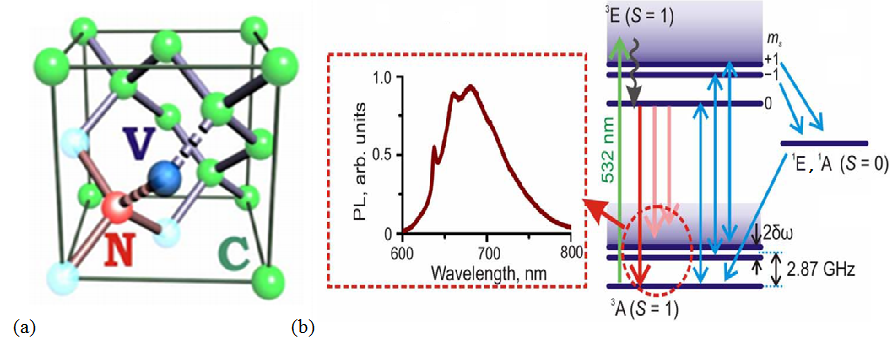
\includegraphics[width=0.8\textwidth]{Figures/NVBackgroundFigure.png}
\caption{(a) A nitrogen atom (N) and a vacancy (V) forming an NV center in a diamond lattice, consisting of carbon
(C) atoms. Four possible arrangements of the NV axis with respect to the crystal lattice of diamond are shown. (b)
Diagram of energy levels involved in electron-spin spectroscopy. The ground state of NV$^-$ is a
spin-triplet state with a zero-field splitting $\Omega_s\approx2.87\unit{GHz}$. When tuned to the ESR frequency $\Omega_s$, a microwave
field efficiently transfers population from the $m_s = 0$ to the $m_s = \pm1$ state. An optical pump at $532\unit{nm}$ couples
the $^{3}A_{2}$ ground electronic state to the $^{3}E$ excited state, giving rise to photoluminescence, shown by the red line,
featuring a characteristic zero-phonon line at approximately $637\unit{nm}$, which is observed in the spectrum of
photoluminescence (shown on the left) against a broad phonon-sideband line, stretching down to $800\unit{nm}$. An
external magnetic field removes the degeneracy of the $m_s = \pm1$ state and induces a Zeeman frequency shift
$2\delta\omega$ between these
sublevels. A substantial fraction of the $m_s = \pm1$ excited-state population is transferred to the $m_s = 0$
ground level via a metastable 1E singlet state.}
\label{NVBackgroundFig}
\end{figure}

\begin{figure}
\centering
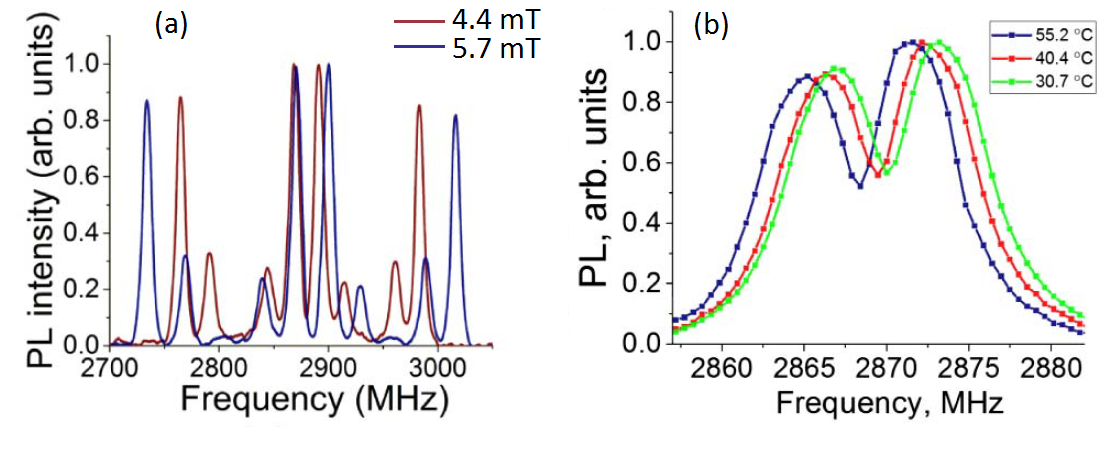
\includegraphics[width=0.8\textwidth]{Figures/TempMag.png}
\caption{Previous ODMR measurements. (a) Shown is the spreading of the 8 ODMR peaks due to an external magnetic field. (b) Plot showing the shift of the ODMR peaks due to a change in external temperature. This shift was measured to be $-75\unit{kHz/K}$.}
\label{TempMag}
\end{figure}

The electron spin of the NV ground-state triplet can be manipulated by a microwave field via electron spin
resonance (ESR). The spin part of the electron Hamiltonian of an NV center in the presence of an external magnetic
field B is written as $H_s=\mu_B g\mathbf{B}\cdot\mathbf{S}+hD[S_z^2-(S(S+1))/3]+hE(S_x^2-S_y^2)$, where 
$\mu_b$ is the Bohr magneton, $g\approx 2$ is the electron g-ratio, $D$ and $E$ are the zero-magnetic-field
splitting parameters, and $S_j \ (j = x, y, z)$ are the projections of the electron spin $S$ on the principal
Cartesian coordinate axes $x, y, z,$ with the z-axis chosen along the NV axis. The first term in this Hamiltonian
describes the Zeeman effect in an external magnetic field, which is observed against zero-field splitting due to
spin-spin interactions in the vacancy site.  This zero field splitting is governed by the second and third terms
in $H_s$, dominated by the splitting $\Omega_s = D \approx 2.87\unit{GHz}$ (where h is the Planck constant) between the $m_s = 0$ spin state
and the twofold-degenerate $m_s = \pm1$ state (Fig. \ref{NVBackgroundFig}b).  When the microwave field is tuned to the ESR frequency $\Omega_s$,
this microwave field efficiently transfers population from the $m_s = 0$ to the $m_s = \pm1$ state (Fig. \ref{NVBackgroundFig}b), thus
manipulating spin orientation. For NV$^-$ in the $m_s = \pm1$ state, the photoluminescence yield is lower than
that typical of NV$^-$ in the $m_s = 0$ state.  This is because a substantial fraction of the $m_s = \pm1$ excited
state population is transferred to the $m_s = 0$ ground level via a metastable singlet state ($^{1}E$ state in Fig. \ref{NVBackgroundFig}b).
This pathway is non-radiative, therefore allowing optical detection of ESR by reading out the spin state from the
intensity of the photoluminescence signal. An external magnetic field $\mathbf{B}$ removes the degeneracy of the
$m_s = \pm1$ state and induces a Zeeman frequency splitting $\Delta\Omega{Z}$ between the $m_s = \pm1$ sublevels (Fig. \ref{NVBackgroundFig}b). Since the
photoluminescence from $m_s = \pm1$ levels is weaker than the photoluminescence from $m_s = 0$ states, the Zeeman-shifted
sublevels are observed as B-dependent features in the ODMR spectrum measured as a function of the microwave
frequency $\Omega$.  The ODMR spectrum changes as a function of applied magnetic field and as a function of NVD temperature.  As the magnetic field increases, the projection of the magnetic field onto the four quantization axes present in a bulk NVD will induce shifts in the corresponding eight ODMR peaks present (one for each spin sublevel in each of four quantization axes), causing the peaks to spread apart (Fig. \ref{TempMag}a).  Temperature manifests as strain in the NVD lattice, and the effect of this strain is to shift the zero-field splitting (parameter D) by -75 kHz/K (Fig. \ref{TempMag}b).

The NV$^0$ charge state is accessable from the NV$^-$ via photoionization of the electron in the vacancy site into the conduction band from the ground state with either a direct single-photon ionization regime or two-photon ionization regime using the excited state as an intermediate transition.  The separation of the NV$^-$ ground state from the edge of the conduction band is approximately 2.6 eV (476 nm); the separation of the singlet state from the conduction band edge is not certain.  The NV$^0$ charge state itself possesses a broad fluorescent transition with a zero phonon line at 575 nm.  Once the NV$^-$ is ionized, it is possible to convert the NV$^0$ back into an NV$^-$ by a two-photon recombination regime.  The NV$^0$ is excited into the $^2$A$_1$ excited state with 532 nm radiation which also pulls an electron from the valence band into the $^2$E ground state, converting the NV$^0$ back into an NV$^-$.

\begin{figure}
\centering
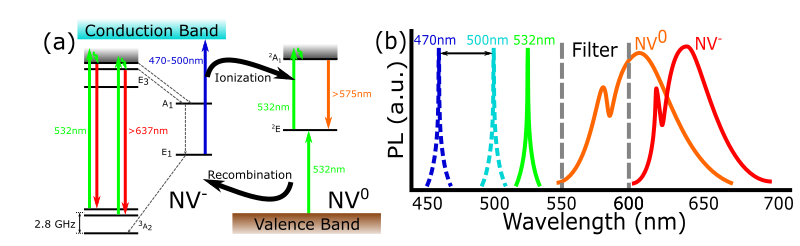
\includegraphics[width=1.0\textwidth]{Figures/IonizationEnergyandFilter.png}
\caption{(a) Energy level diagrams of NV$^-$ and NV$^0$ states. Shown are the range of singlet ionization wavelengths from $470-500\unit{nm}$ that we will attempt to ionize the singlet state with, and the $532\unit{nm}$ NV$^0$ recombination wavelength. (b) Photoluminescence of both the NV$^-$ and NV$^0$. The filter bandwidth that isolates the NV$^0$ signal from the NV$^-$ and pump and probe lasers is shown.}
\label{IonizationEnergyandFilterFig}
\end{figure}

The proposed research is aimed at advancing the fundamental understanding of the NV singlet state that will
inspire new and novel high contrast optical, temperature, and magnetic field imaging techniques.  As a part of
the proposed research program, we plan to achieve the following goals:
\begin{enumerate}
\item Use selective ionization of the NV$^-$ from the singlet state to determine the separation between the singlet state and the conduction band edge (Fig. \ref{IonizationEnergyandFilterFig}a).
\item Develop a technique for enhanced contrast ODMR that involves tying the NV$^-$ spin state to the population in the NV$^0$ state via selective photoionization of the NV$^-$ singlet state.
\item Leverage the enhanced contrast ODMR technique to improve the temperature and magnetic field sensitivity of our fiber NVD probes for the purpose of deep tissue weak field diagnostics.
\item Determine the dependence of ODMR contrast on the NVD temperature and on the wavelength of IR radiation targeted at the transition in the singlet manifold.
\item Develop a novel temperature sensitive STED technique immune to background autofluorescence.
\end{enumerate}

Correspondingly, the proposed activities are divided into the following work packages (WP): NV singlet 
ionization (WP1), enhanced contrast ODMR (WP2), enhanced sensitivity fiber NVD probes for deep tissue weak field 
diagnostics (WP3), characterization of ODMR dependence on temperature and IR radiation (WP4), and temperature 
sensitive super-resolution STED imaging (WP5). Wherein the stated goals of the WP1-3 motivate each 
subsequent work plan (Fig. \ref{WP12345FlowChart}a). Also, the results for WP4 provide the preliminary results 
for WP5 (Fig. \ref{WP12345FlowChart}b)

\subsection{WP1: NV Singlet Ionization}
\begin{figure}
\centering
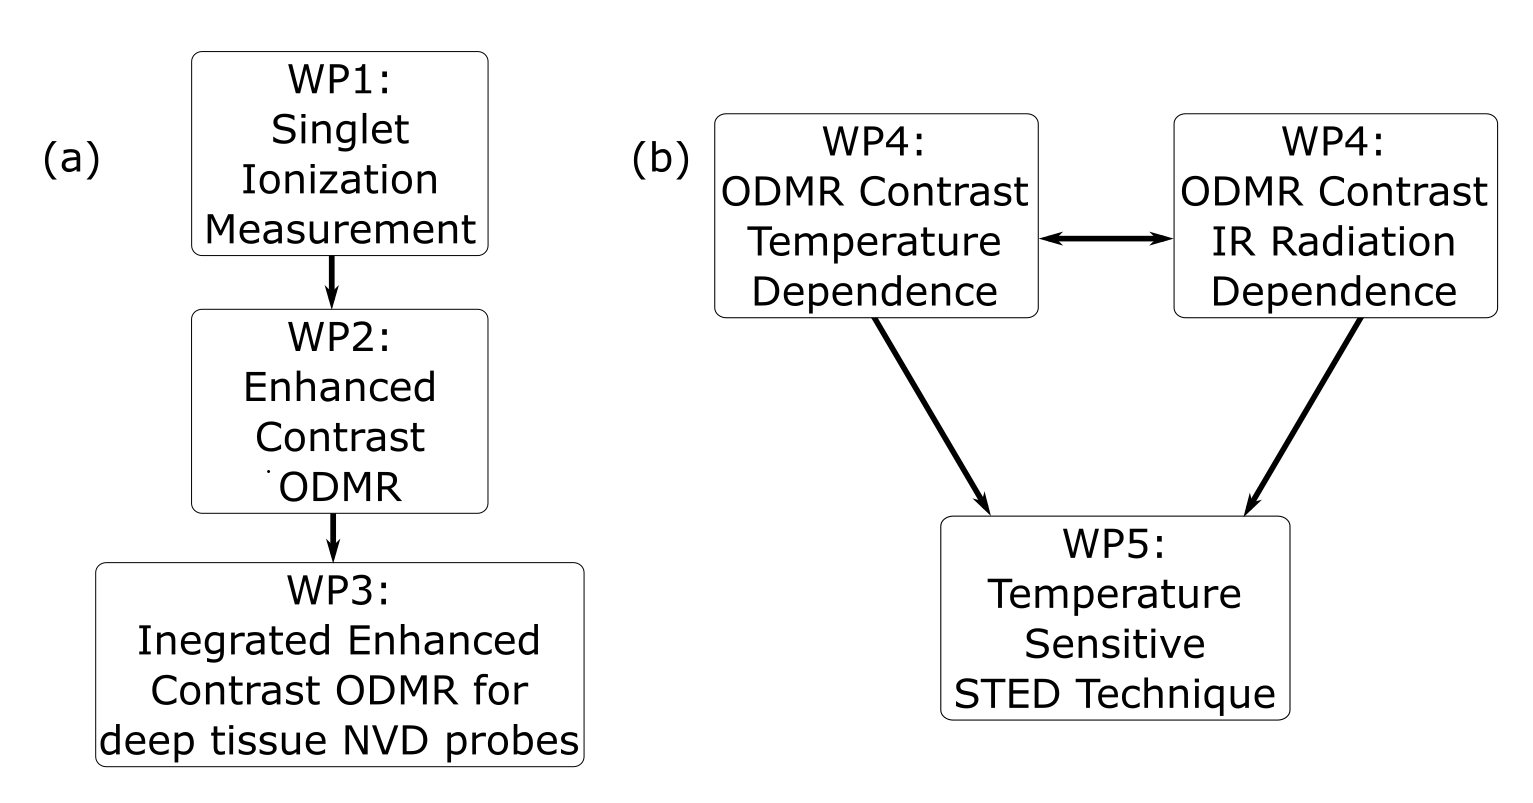
\includegraphics[width=0.8\textwidth]{Figures/WP12345FlowChart.png}
\caption{Work plan flow diagram for progression of experimental activities from WP1 to WP3}
\label{WP12345FlowChart}
\end{figure}

A deeper understanding of the NV singlet state is a necessity for the development of new applications of the NV
center and for pushing existing measurement regimes into previously inaccessible realms.  In this work package we
intend to demonstrate a technique for ionization of the NV center singlet state.  We plan to use this to measure of the energy separation between the singlet state and the conduction band edge by investigating the fluorescence amplitude of the newly created NV$^0$ as a function of input ionization wavelength.

Our experimental plan to accomplish this goal will involve pumping the NV center into the singlet state by first spin
polarizing the NV center into the $m_s = 0$ ground state sublevel with a pulse of $532\unit{nm}$ laser
excitation
lasting not more than the lifetime of the singlet state ($\sim200\unit{ns}$ at room temperature
\cite{Dreau2011}) from a frequency
doubled Nd:YAG laser modulated with an AOM (Fig. \ref{WP1Schematic}).  We will then populate the singlet
state with a microwave
$\pi$-pulse resonant with the ground state Zeeman splitting followed by another $532\unit{nm}$ laser
pulse with a duration of
$100\unit{ns}$ (approximately 10 excited state lifetimes) to ensure the population has a chance to
transition into the
singlet state via its 50\% ISC with the $m_s = \pm1$ excited state sublevels.  We will then immediately apply a
short, intense
probe ionization pulse with variable wavelength from $470-500\unit{nm}$ (Fig. \ref{IonizationEnergyandFilterFig}a), followed by a third $532\unit{nm}$ pulse with
$200\unit{ns}$ duration that
will detect a charge in charge state of the NV center by 
exciting the NV$^0$ and collecting the fluorescence.  This pulse will also serve to re-polarize the NV center into the $m_s = 0$ state should
ionization
not have occurred, and will convert an NV$^0$ back into an NV center and re-polarize it in the event
that it had ionized.

\begin{figure}
\centering
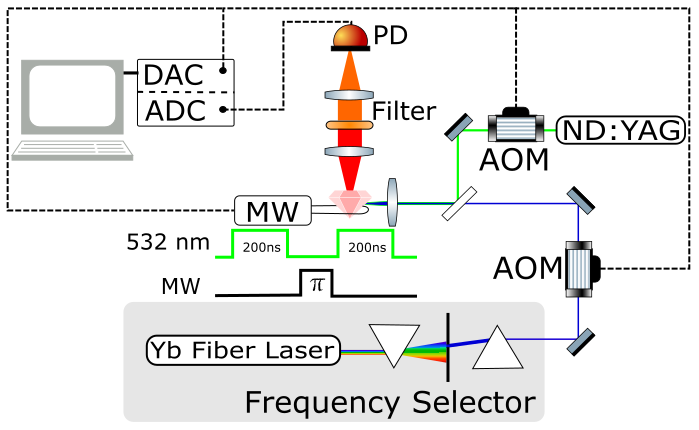
\includegraphics[width=0.8\textwidth]{Figures/WP1Schematic.png}
\caption{Experimental Schematic for WP1. A computer controlled DAC controls the pulse regime to sync the microwave (MW) and the two light sources. We use a prism pair to frequency select the ionization wavelength from out Yb Fiber Supercontinuum laser. The filter used is described in Fig. \ref{IonizationEnergyandFilterFig}b.  The acousto-optic modulators (AOM) and microwave source are synchronized to the digital to analog controller (DAC) that serves as the driver for these devices.  A pulse train consisting of a 200 ns 532 nm polarization pulse, followed by a microwave Pi pulse targeted at the zero-field splitting 1 microsecond later serves to spin polarize the NV system into one of the $m_s=\pm1$ sublevels.  A second pulse train follows immediately after consisting of a 100 ns 532 nm pulse that shelves the population into the singlet state followed immediately by a 10 ps ionization pulse between 475 nm and 500 nm that will ionize the singlet into the NV$^0$ charge state if it is resonant with the separation between the metastable singlet and the conduction band edge.  A third pulse consisting of a 200 ns 532 nm pulse that recombines and repolarizes the NV$^0$ into an NV$^-$ or repolarizes the NV$^-$ if ionization did not occur.  This pulse will also serve to excite the NV$^0$ should ionization have occured, and the fluorescent output of this excitation will be coupled to a photodiode and read out through our analog to digital converter (ADC).}
\label{WP1Schematic}
\end{figure}

We will repeat this process over a wide range of ionization wavelengths and plot the output of the NV$^0$
fluorescence intensity as a function of input ionization wavelengths.  The singlet state is protected
from two-photon ionization due to the lack of an intermediate state that lies close enough to the
conduction band edge to be ionized by two photons of the same wavelength \cite{Shields2015}.  Thus the
single-photon
ionization events should contribute to a majority of the population in the NV$^0$ charge state, with the
remainder of the population coming from two-photon ionization as a result of the polarization pulse. 
If the polarization pulse power is kept low, then the quadratic nature of the two-photon ionization
rate should contribute a negligible fraction of the NV$^0$ population when compared to the much higher
single photon ionization rate \cite{Aslam2013}.  In this way we can detect the separation between the NV singlet
state and the conduction band edge by measuring the NV$^0$, whose signal is easily separable from both the
signal of the pump and probe pulses and from the NV fluorescence with a simple filter.

\subsection{WP2: High Contrast ODMR}
Building on the results from WP1, we plan to create a technique for radically improved ODMR contrast by
utilizing the ability to map the NV$^0$ fluorescence onto the spin-state of the NV center developed in
WP1.  This technique will exploit a continuous wave ionization regime capable of ionizing from the
singlet state of the NV center and detecting the NV$^0$ as a function of microwave frequency to generate a
high-contrast ODMR spectrum necessary for high-sensitivity vectorial magnetic field measurements.  The
magnetic field sensitivity depends on the ODMR contrast according to the following equation
\cite{Dreau2011}: 
\begin{equation}
\eta_{B} (T\sqrt{Hz}) = P_F\frac{h\Delta\nu}{g\mu_B C\sqrt{R}}.
\label{ODMRSensitivity}
\end{equation}
$P_F$ is an ODMR resonance line-shape parameter, $\Delta\nu$ is the ODMR linewidth,
$C$ is the ODMR contrast, and $R$ is the count rate of fluorescence photons.  From equation \ref{ODMRSensitivity} we can see
that a full contrast ($C=1$) measurement provides more than a factor of three improvement in sensitivity
compared to the best case scenario level of contrast for a traditional ODMR measurement ($C=0.3$) with
the NV center.

\begin{figure}[h]
\centering
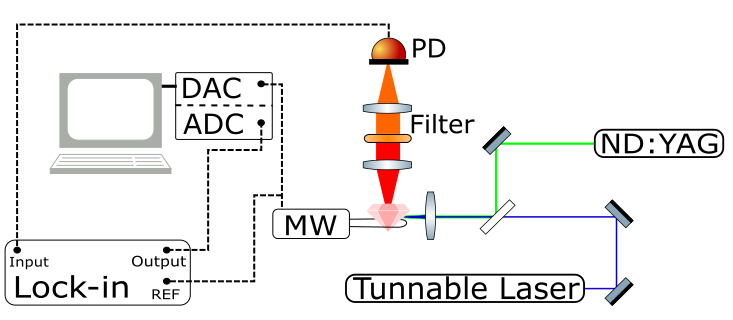
\includegraphics[width=0.8\textwidth]{Figures/WP2Schematic.png}
\caption{Experimental Schematic for WP2. CW 532 nm and adjustable wavelength radiation tuned to the singlet ionization threshold are focused onto an NVD and a 1 kHz amplitude modulated microwave frequency sweep is applied to modulate population in the singlet state.  When the microwave frequency is in resonance with the Zeeman splitting of the ground state sublevels, the singlet state is populated by the 532 nm laser excitation and ionized into the NV$^0$ charge state by the adjustable wavelength radiation tuned to the singlet ionization threshold.  The population in the NV$^0$ charge state fluctuates in phase with the 1 kHz microwave modulation due to the periodic population of the singlet state induced by the modulated microwave energy.  Lock-in detection is used to improve signal to noise ratio of the collected NV$^0$ fluorescence.  As the microwave field is swept in frequency, ODMR fluorescence peaks appear in the plot of NV$^0$ fluorescence as a function of microwave frequency, generating an ODMR spectrum.  The NV$^-$ fluorescence and excitation wavelengths are filtered out with a 50 nm bandpass filter centered on 575 nm for enhanced ODMR contrast.}
\label{WP2Schematic}
\end{figure}

We will accomplish this goal by exciting the NV$^-$ with CW $532\unit{nm}$ laser radiation from our
Nd:YAG source while performing an amplitude modulated microwave frequency sweep to populate the singlet
state (Fig. \ref{WP2Schematic}).  We will simultaneously apply laser radiation with power equal to that of the 532nm
laser radiation and a wavelength targeted at the separation of the singlet state from the conduction
band edge discovered in WP1.  This will facilitate photoionization of the singlet state when the
frequency of the microwave field is at a Zeeman resonance.  The continuous wave $532\unit{nm}$ laser radiation
will excite the population in the NV$^0$  state and provide fluorescent readout as a function of applied
microwave frequency, generating an ODMR spectrum when filtered from the NV center fluorescence and pump
excitation.  A CW regime with laser powers on the scale of $1\unit{mW}$ is necessary to ensure dominance of
single-photon ionization when applied to an NVD with a high density of NV$^-$ centers for improved ODMR contrast and to ensure sharp ODMR resonances and reduced
laser heating for enhanced sensitivity.  Lock-in detection referenced to the amplitude modulated
frequency of the microwave sweep will enhance signal collection.

\subsection{WP3: Enhanced Sensitivity Fiber NVD Probes for Deep Tissue Weak Field Diagnostics}
Integration of NV quantum sensors with optical fibers is tremendously beneficial for a broad class of
applications of NV-center-based magnetometry, including high-resolution, high sensitivity deep tissue
bio-medical diagnostics. As a part of the earlier work in this direction, a variety of technologies
enabling the embedding of diamond nanoparticles with NV$^-$ into specially designed optical fibers
have been developed and ultracompact fiber-optic probes integrating NV quantum sensors with a waveguide
delivery of optical and microwave fields have been demonstrated. In this work package we intend
incorporate the photoionization enhanced ODMR contrast technique developed in WP2 into our existing
fiber-optic NVD techniques in order to improve performance characteristics of these fiber-optic NVD
probe. We will use commercial diamond microcrystals, enriched with NV defects to an NV density of up to
$n \approx 10^{15}-10^{16}\unit{cm^{-3}}$ by irradiation with MeV electrons and high temperature annealing. 
These microcrystals will be deposited on the tip of a fiber-optic probe (Fig. \ref{WP3Schematic}) with a mechanical 
manipulator under an optical microscope and attached to the fiber tip with ethyl cyanoacrylate glue.

\begin{figure}[h]
\centering
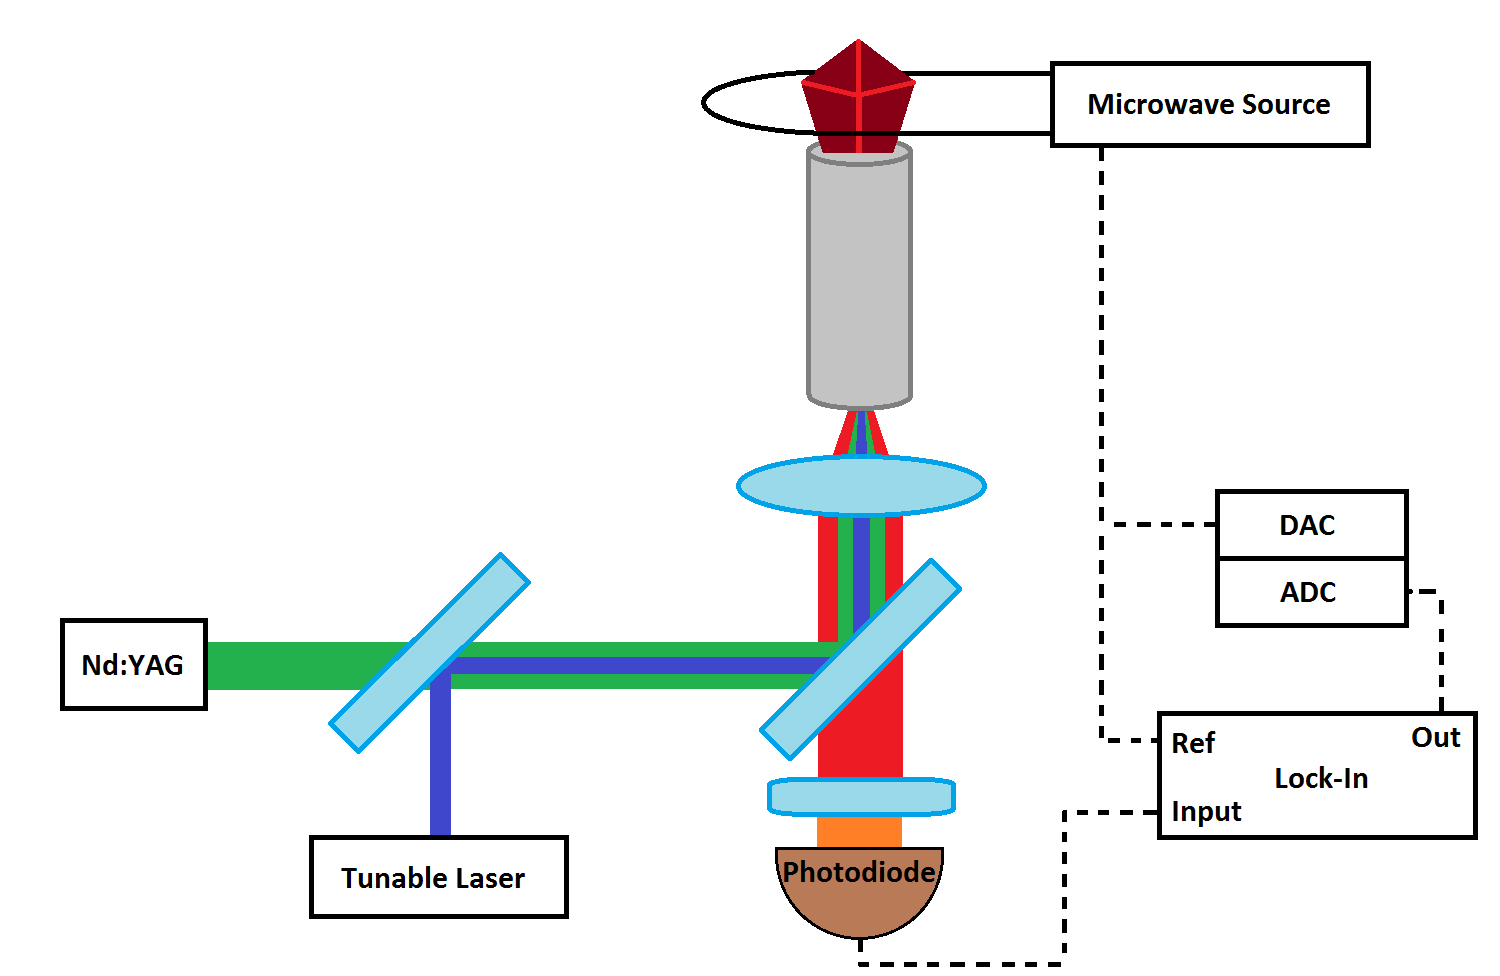
\includegraphics[width=0.8\textwidth]{Figures/DualFiberWP3Image.png}
\caption{Experimental Schematic for WP3. In this experiment we adapt the experimental setup as described in WP2 by integrating a NVD attached to a fiber optic cable tip. We use the fiber optic cable to carry the 532 nm pump laser and the tunable probe laser light to the NVD. The florescent signal is returned through a band pass filter to the be detected on a photodiode down the same fiber.}
\label{WP3Schematic}
\end{figure}

The amplitude modulated microwave excitation needed for the photoionization assisted ODMR technique developed in WP2 will be 
delivered to the diamond microcrystal with NV$^-$ through a two-wire transmission line, running along the 
optical fiber and consisting of a pair of copper wires terminated by a loop around the NVD placed at the fiber 
tip.  Optical initialization of NV$^-$ will be delivered to the diamond microcrystal on the fiber tip through 
the core of the fiber probe. The fluorescence emitted by the NVD will be coupled back into the probe, 
and returned through the fiber to the detection system, consisting of a silicon photodiode and a lock-in 
amplifier.  We will take multiple measurements of the magnetic field or the temperature at a grid of points 
around the object of interest and generate spatial magnetic field map or spatial temperature distribution of the 
object under study. 

\subsection{WP4: Characterization of ODMR dependence on temperature and IR radiation}

Differentiating between the effect of temperature and the wavelength of incident IR radiation on ODMR contrast 
is of paramount importance in the development of temperature sensitive super-resolution STED microscopy.  In 
this work package, we plan to achieve this goal with two experiments. 

The first experiment in this work package will involve determining the dependence of the ODMR contrast on
temperature. We propose to accomplish this by exciting the NVD with CW 532 nm laser radiation and microwave
radiation resonant with the zero-field ground state splitting.  We will attach the diamond to a thermocouple and
apply a heat source to the NVD.  We will plot the fluorescence signal from the NVD as a function of temperature
to determine the effect of temperature on ODMR contrast. This experimental setup is shown in Fig. 
\ref{WP4TempSchematic}.

\begin{figure}
\centering
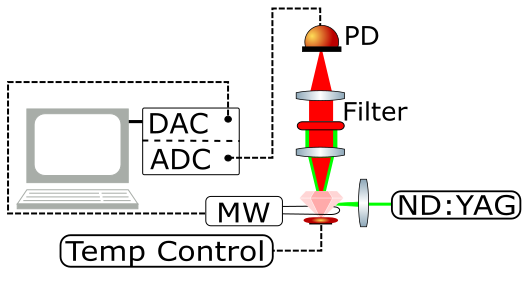
\includegraphics[width=0.7\textwidth]{Figures/WP4TempSchematic.png}
\caption{The experimental schematic for probing the temperature response of ODMR contrast in WP4. A 532 nm CW pump laser is focused onto a NVD thereby inducing excitation. A microwave transmission line carries the microwave frequency targeted at the zero-field ground state splitting. A thermocouple with an electronically controlled Thermoelectric cooling (TEC) element electronically controls the temperature of the NVD at a known temperature. The TEC and thermocouple system allows for variable temperature control providing the temperature response of the ODMR. The NV$^-$ fluorescence is collected on a photodiode through a 200 nm band pass filter between 650 nm and 850 nm so that the fluorescent signal is isolated from the 532 nm pump wavelength. The ODMR contrast is then plotted as a function of temperature.}
\label{WP4TempSchematic}
\end{figure}

The second experiment will involve determining the dependence of the ODMR contrast on the wavelength of incident
IR radiation.  We propose to accomplish this by again exciting the NVD with CW 532 nm laser radiation and
microwave radiation resonant with the zero-field ground state splitting, and then applying laser excitation from
a broadband IR laser.  We plan to test the dependence of the ODMR contrast on IR wavelengths between 900 nm and
2200 nm by focusing the output of a supercontinuum Yb fiber laser coupled to a 1 nm FWHM bandwidth monochromator
onto the NVD and then plotting the fluorescence signal as a function of IR wavelength applied to the NVD in 
order to determine the effect of the wavelength of IR radiation on ODMR contrast. This experimental setup is 
shown in Fig. \label{WP4IRSchematic}.

\begin{figure}
\centering
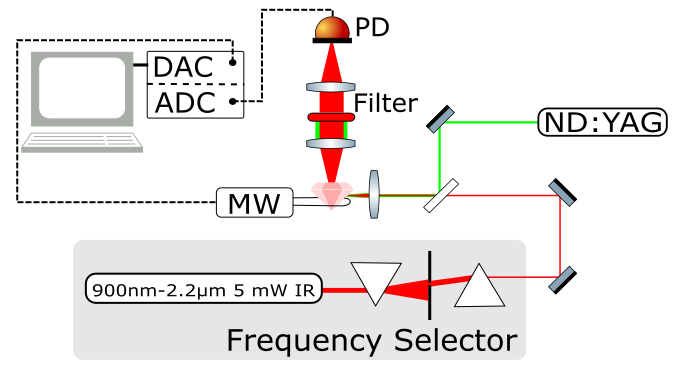
\includegraphics[width=0.8\textwidth]{Figures/WP4IRSchematic.png}
\caption{Experimental schematic for probing the IR response of ODMR contrast in WP4.  532 nm CW laser excitation and fixed power variable IR laser wavelengths are focused onto the diamond.  A microwave transmission line applies microwave radiation modulated in amplitude at 1 kHz with frequency targeted at the zero-field splitting to the diamond.  The IR laser power is fixed at a level that reduces the ODMR contrast by 50\% due to IR heating of the NVD and the wavelength is tuned between 900 nm and 2200 nm.  The NV$^-$ fluorescence is coupled to a photodiode through a 200 nm band pass filter between 650 nm and 850 nm in order to isolate only the NV$^-$ fluorescence signal.  The ODMR contrast is thus plotted as a function of input IR wavelength.}
\label{WP4IRrSchematic}
\end{figure}

\subsection{WP5: Temperature sensitive super-resolution STED imaging}
In this work package we plan on leveraging the information gained about the dependence of the ODMR contrast on 
temperature to create a novel temperature sensitive STED regime.

	We plan to implement this regime by using a microscope objective to simultaneously focus 532 nm onto a high-
density NVD with integrated microwave transmission lines supplying pulsed microwave excitation with frequency 
targeted at the NV$^-$ zero-field splitting for amplitude modulation of NV$^-$ fluorescence.  This technique 
will produce bright NV$^-$ fluorescence with modulated intensity at a depth of up to 30\%.  We will then apply 
an 815 nm torus shaped beam formed using a spatial light modulator (SLM) to overlap the region illuminated with the 532nm radiation in order to induce 
stimulated emission depletion of the NVD fluorescence for super-resolution imaging.  The non-depleted, modulated 
fluorescence amplitude of the central region will be collected using a lock-in amplifier referenced to the pulse 
repetition rate of the microwave radiation to separate the background fluorescence from the desired signal.  The 
amplitude of the collected signal will be proportional to the change in temperature due to the dependence of the 
ODMR contrast on NVD temperature discovered in WP4.  This measurement will be repeated over the entire surface 
of the object under study using a 3-axis motorized translation stage in order to generate a super-resolution 
image of the object with an overlay of the spatial temperature distribution. 

\begin{figure}
\centering
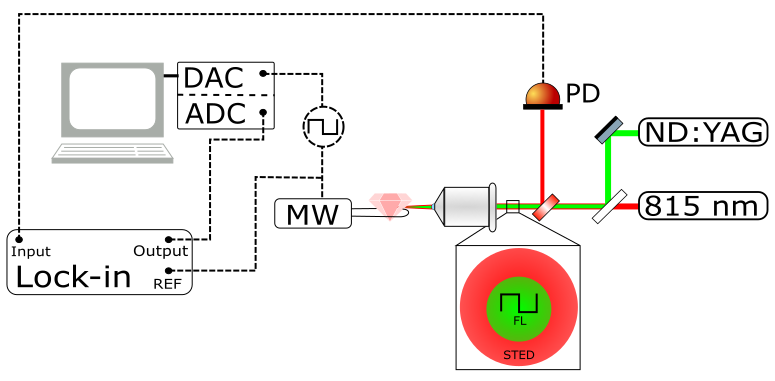
\includegraphics[width=0.8\textwidth]{Figures/WP5Schematic.png}
\caption{The experimental schematic for WP5.  A 5 mW 532 nm CW laser excitation is coupled through an objective and onto a diamond sample with an integrated microwave transmission line.  A torus-shaped spatial mask is applied to a 30 mW CW 815 nm laser beam using a spatial light modulator (SLM).  This beam is overlaid onto the same spot on the diamond as the 532nm excitation via the objective and drives down the NVD fluorescence via stimulated emission depletion.  The microwave source provides lock-in referenced amplitude modulated microwave excitation targeted at the NV$^-$ zero-field splitting in order to modulate the the unsuppressed NVD fluorescence.  The amplitude of modulation of the unsuppressed fluorescence is the ODMR contrast, which is dependent on the temperature of the NVD.  We image the modulated temperature sensitive ODMR contrast at many points on an x-y grid using a three axis translation stage onto a photodiode and use lock-in detection to separate the desired signal from noise and generate a back-ground fluorescence free temperature sensitive super-resolution image of our NVD.}
\label{WP5rSchematic}
\end{figure}

\section{Mechanisms to Assess Success}
The success of the research under the five work packages will be assessed by the following criteria:
\begin{itemize}
\item The success of the work under WP1 will be judged by a proof of principle demonstration of NV$^-$ singlet ionization whereby we will measure a peak in NV$^0$ fluorescence as a function of input ionization wavelength when the system is prepared in the singlet state.
\item The success of work under WP2 will be judged by demonstration of ODMR contrast greater than 30\% by measuring NV0 fluorescence amplitude as a function of input microwave frequency in the CW singlet photoionization regime.
\item The success of work under WP3 will be judged by demonstration of up to a factor of three higher magnetic field sensitivity using the photoionization ODMR technique described in WP2 when compared to the standard ODMR technique.
\item The success of work under WP 4 will be judged by demonstrating a graph of the dependence of ODMR contrast on temperature between 300K and 400K and a graph of the dependence of ODMR contrast on the wavelength of IR excitation between 900 nm and 2200 nm.
\item The success of work under WP5 will be judged by demonstrating high contrast imaging of heated NVD particles under 250 nm in diameter against a bright fluorescent background while simultaneously measuring their temperature.
\end{itemize}

\section{Intellectual Merit}
A better understanding of the singlet state energy level structure is of broad interest 
across the many applications of NVDs. Our work directly affords the possibility of quantum 
sensors with radically enhanced sensitivity to magnetic fields and temperature 
distributions.  Enhanced knowledge of the dependence of ODMR contrast on temperature will 
give rise to the prospect of temperature sensitive super-resolution imaging immune to 
background autofluorescence. The proposed measurement techniques will resolve important 
open questions about the NV$^-$ singlet state energy level structure and illuminate the 
previously unexplained dependence of the ODMR contrast on temperature and the wavelength of 
infrared excitation.

\section{Broader Impact}
Using existing fiber platform NVD probe technology, ultra-high sensitivity fiber 
magnetometers and thermometers with submicron resolution are possible.  These probes can be 
used for in vivo magnetic field and temperature diagnostics of previously inaccessible deep 
tissue environments that are relevant to real-time spatially resolved magnetic imaging of 
individual neuron action potentials and sensitive subcellular thermometry necessary for the 
characterization of in vivo intracellular reaction kinetics.  By measuring the dependence 
of ODMR contrast on temperature, a novel temperature sensitive STED regime immune to 
background fluorescence can be developed to create nanoscale resolution temperature 
resolved fluorescence images as a tool for new paradigms in medical diagnostic imaging.

\section{Results from Prior NSF Support}
Not Applicable.

\bibliographystyle{unsrt}
\nobibliography{2017NSF}

\end{document}
